\section{Introduction}
The goal of the project work was to implement a peripheral driver for the STM32f407 microcontroller. The implemented driver enables the use of the analog-to-digital converter (ADC). The microcontroller which contains the analog-to-digital converter is located on a development board (STM32 F4 Discovery kit) shown in figure \ref{fig:Board}. This development board contains components that can be interfaced with the microcontroller.\\

\begin{figure}[htbp]
  \centering
     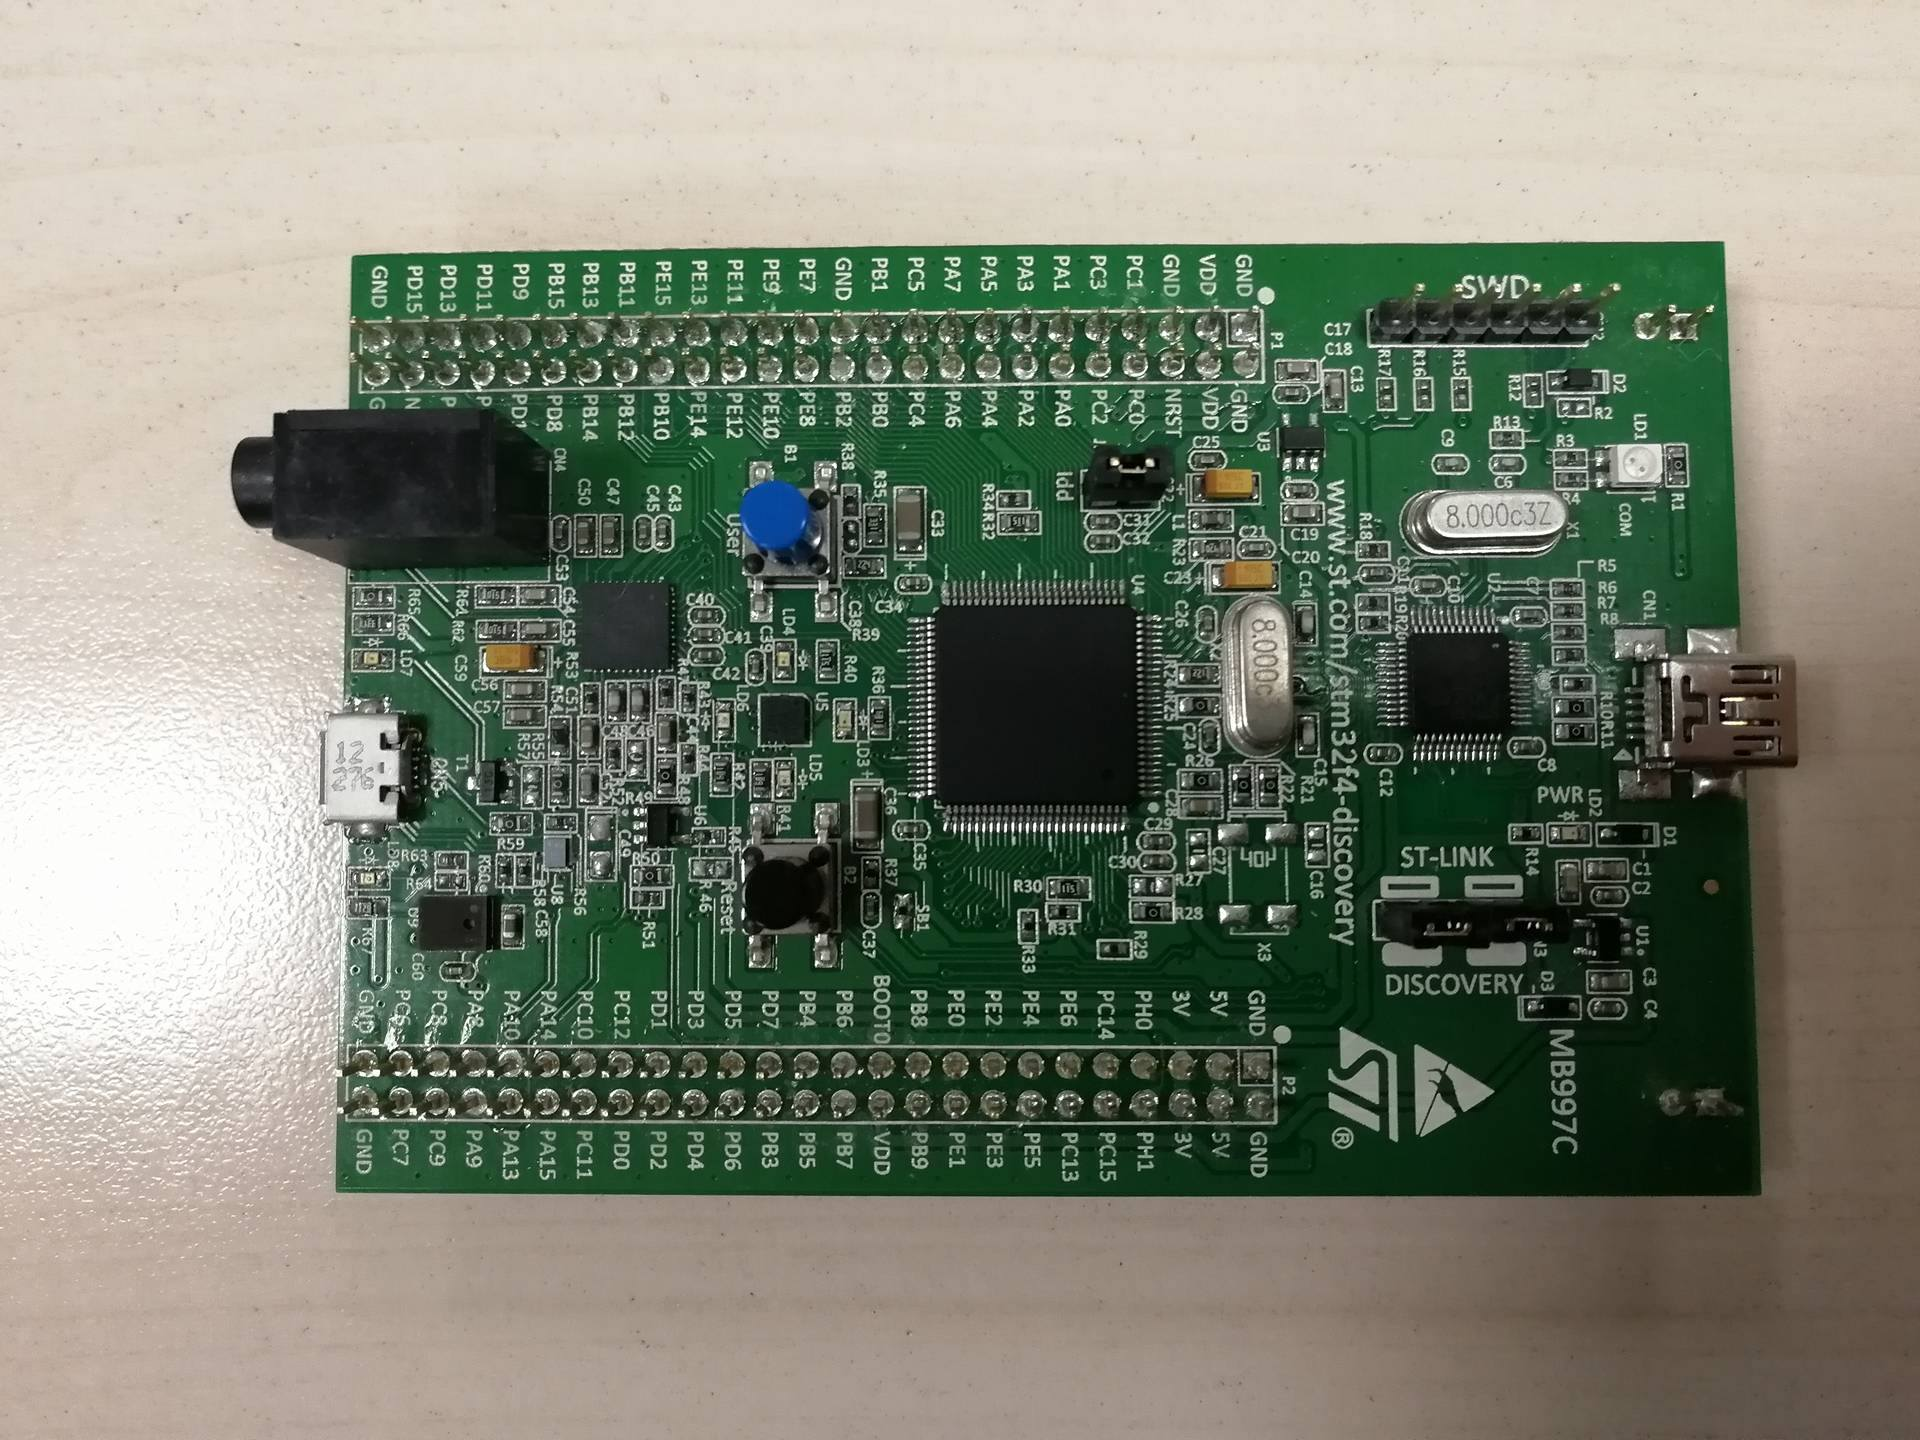
\includegraphics[width=0.7\textwidth]{./figures/board.jpg}
  \caption{Discovery Board}
  \label{fig:Board}
\end{figure}

\begin{figure}[htbp]
  \centering
     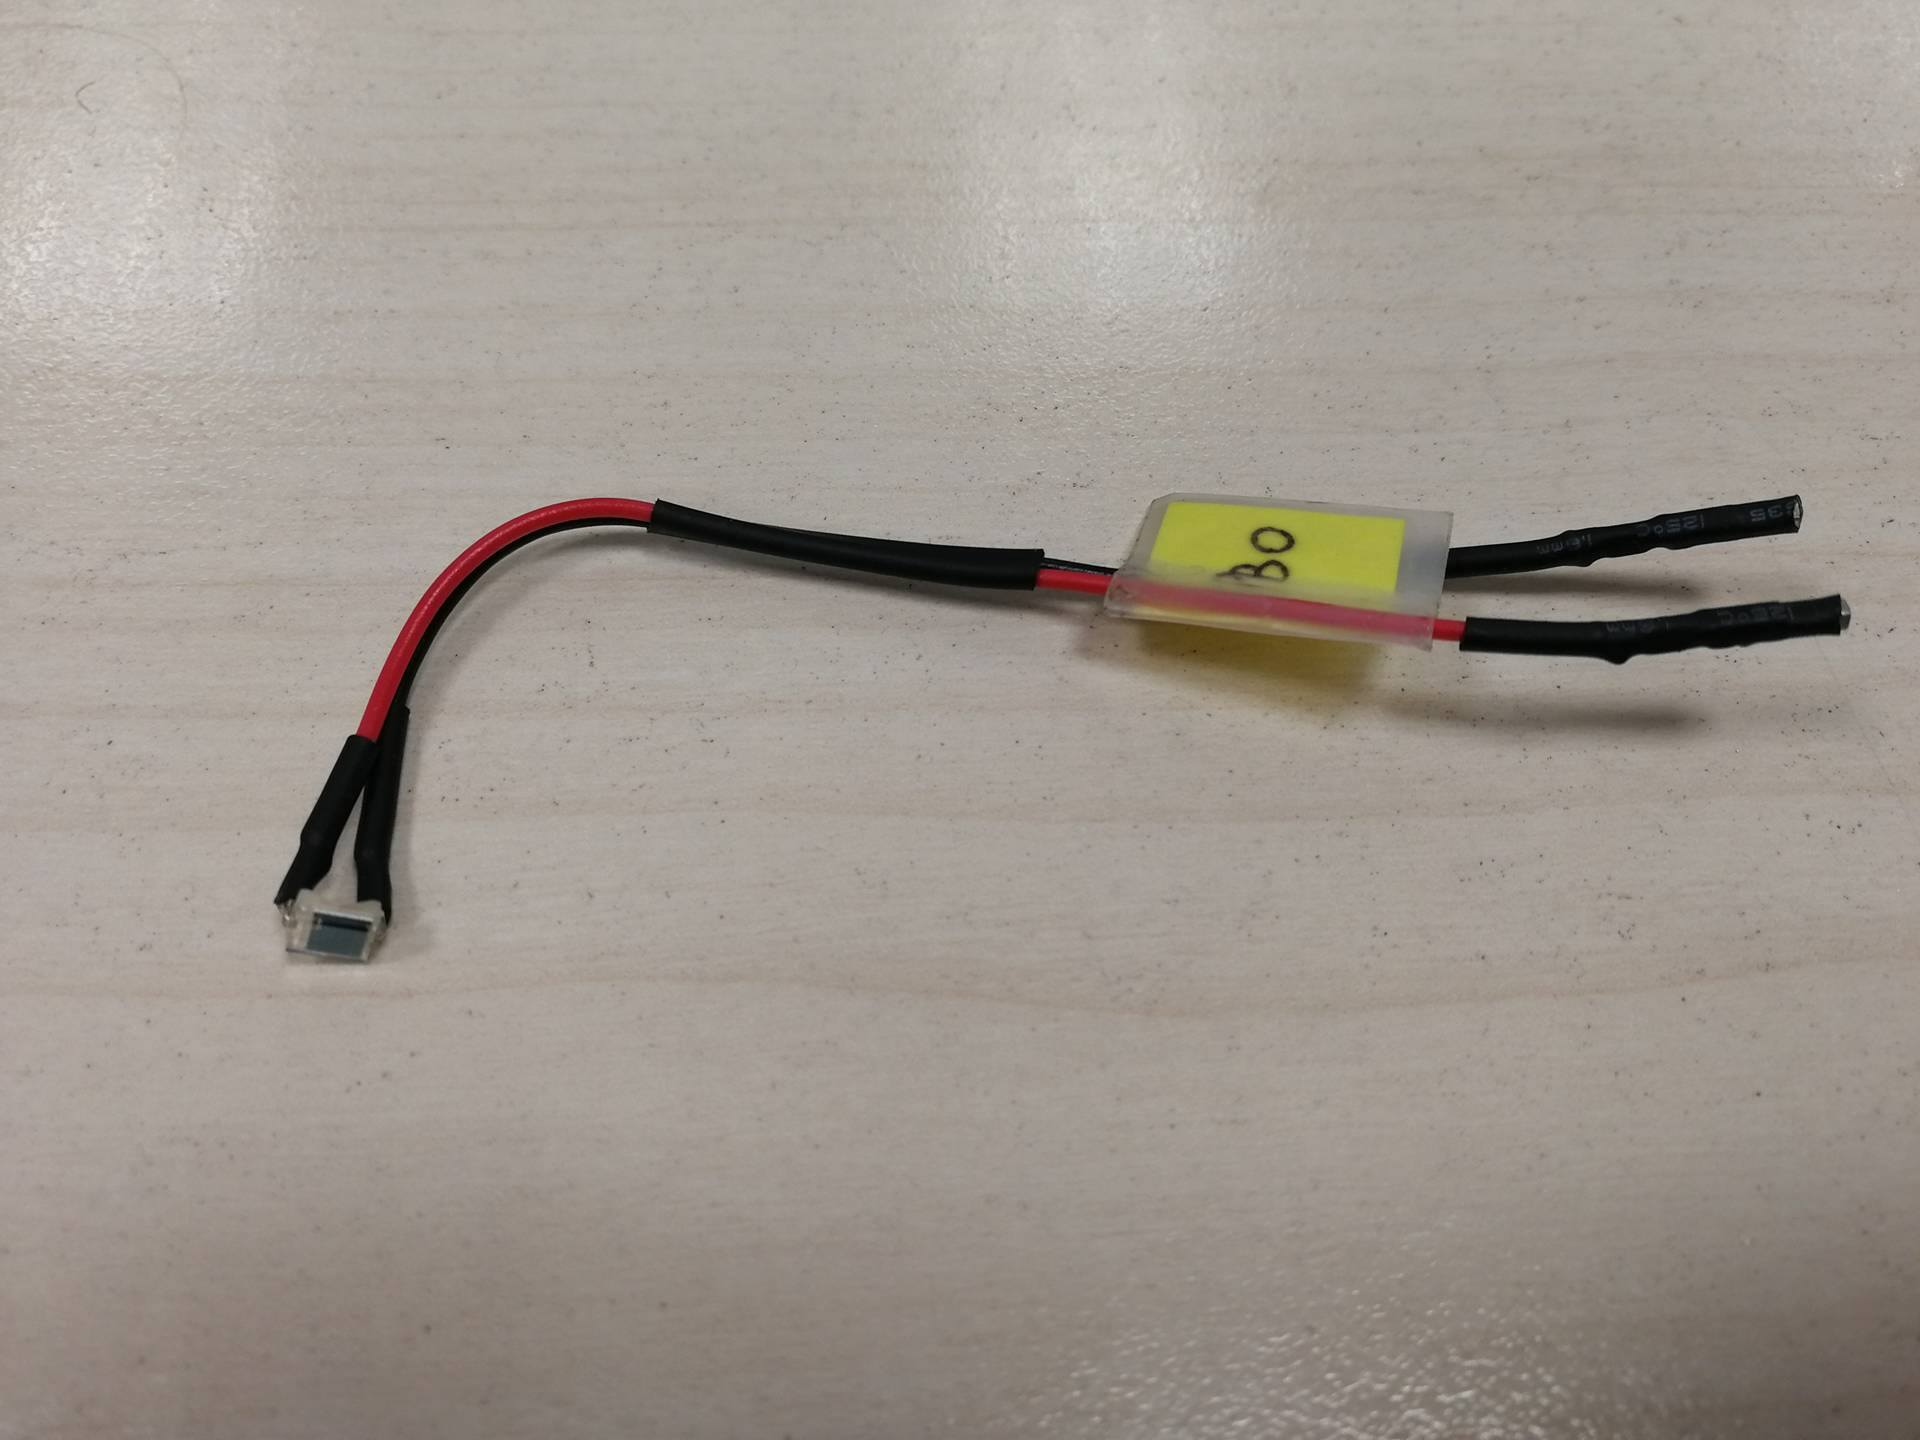
\includegraphics[width=0.5\textwidth]{./figures/photodiode.jpg}
  \caption{Photodiode}
  \label{fig:photodiode}
\end{figure}

\par
In this work the push buttons and LEDs were utilized. An external photodiode shown in figure \ref{fig:photodiode} was connected to the development board connection pins. These components were used to make a simple user reaction game.

\pagebreak


\section{Design and implementation}
\subsection{Game logic}
The idea of the implemented game was to test the reaction time of a player. This game can be played by a defined number of players. The reaction time of a player is evaluated by indicating a start signal and after this signal the player has to cover the photodiode as fast as possible. The game logic is illustrated in figure \ref{fig:GameLogicDiagram}. 

\begin{figure}[htbp]
  \centering
     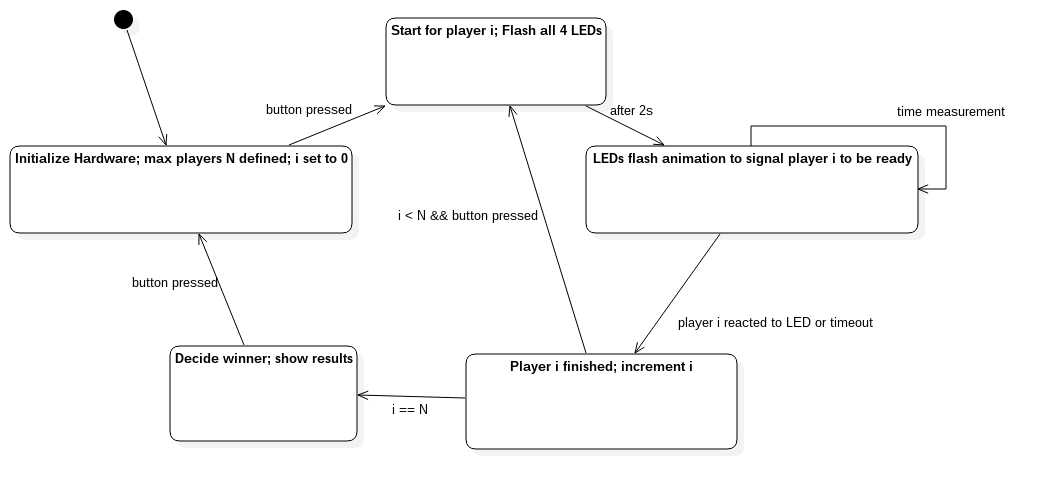
\includegraphics[width=1\textwidth]{./figures/FSM_Diagram.png}
  \caption{Game logic diagram}
  \label{fig:GameLogicDiagram}
\end{figure}

As illustrated in figure \ref{fig:GameLogicDiagram} the game is started after the hardware initialization has been completed. This is done when the power of the board is turned on and the board's push button has been pressed. Information about the game status and corresponding instructions are printed on a serial monitor. These instructions are shown in chapter \ref{Results}.\\
\par
After the push button has been pressed it is the first player's turn and all of the user programmable LEDs start to flash rapidly for a short duration and then turn off. This is an indication to the player to get ready to get ready. After this the LEDs start to light up in a clockwise orientation one by one. Once the fourth LED has lighten up, the player has to cover the photodiode as quickly as possible. Player reaction time is measured from the fourth LED lighting up and to the point when the photodiode has been covered.\\ 
\par
Then another player starts their turn by pressing the push button and has to interact in the same manner as the player before. This cycle is repeated until all of the players have had their turn. The reaction times are finally displayed and the player who had the lowest reaction time wins the game. A new game can be started by pressing the push button.

\subsection{Peripheral drivers}
For simplicity a design choice for this microcontroller project was to avoid the use of threads. Every game logic procedure is executed in a sequential order and only interrupts allow to break this cycle and trigger events concurrently.\\
\par
In this project, interrupts are used by timers to toggle LEDs and for button detection. For the analog watchdog polling is utilized.
This approach allows to sense if the user tries to cheat by covering the photodiode before the fourth LED start to flash. As an alternative to this it would be also possible to realize the watchdog with interrupts and toggle the LEDs with sleep delays.\\
\par
The Miosix operating system (\cite{Miosix}) is included in the project workspace and is mainly used for a simplified accessing of the STM32F4 peripheral addresses by calling provided register names. Also the \emph{Timer} class for measuring time and the \emph{Random Number Generator} are exploited.

\subsubsection{ADC}
The control of the analog-to-digital converter builds the core of the project. A simple photodiode is connected to the board and introduces an analog input voltage level depending on the ambient light intensity. The voltage has to be detected and read out as a digital signal in defined time intervals. Since the actual values are not important for this project, there is no data processing necessary. The values simply have to be compared to a threshold voltage and if they exceed this threshold, further action should be initiated. The analog watchdog provided by the microcontroller is used to execute this comparison.

%TODO Arno
%explain with the registers how the adc is actually used
%explain calibration

\subsubsection{Push button}
%TODO Arno

\subsubsection{LEDs \& Timer}
Since the toggling of the LEDs is realized with interrupts, the LED management explicitely includes a hardware timer. The \emph{Led} class knows three different operating modes: At the beginning of a game round all four LEDs flash rapidly, after that the number of blinking LEDs increase from 1 to 3 and finally after a random time interval also the fourth LED becomes active. For all these three modes only one timer (TIM3) needs to be utilized because the blinking procedures happen sequentially.\\
\par
For every sequence the function \emph{startLedTimer()} is called with a different time interval which sets the prescaler of the timer. Also the new LED mode is passed with the function. With the given mode every time the timer generates an overflow interrupt, the corresponding IRQ handler knows in which way the LEDs should be toggled.

\subsubsection{Serial}
%TODO Arno
%black GND (not necessary?), yellow PB10, orange PB11
%sudo screen /dev/ttyUSB0 19200

\subsubsection{Connections}
%TODO Arno

\cite{RefManual}
\begin{figure}[htbp]
  \centering
     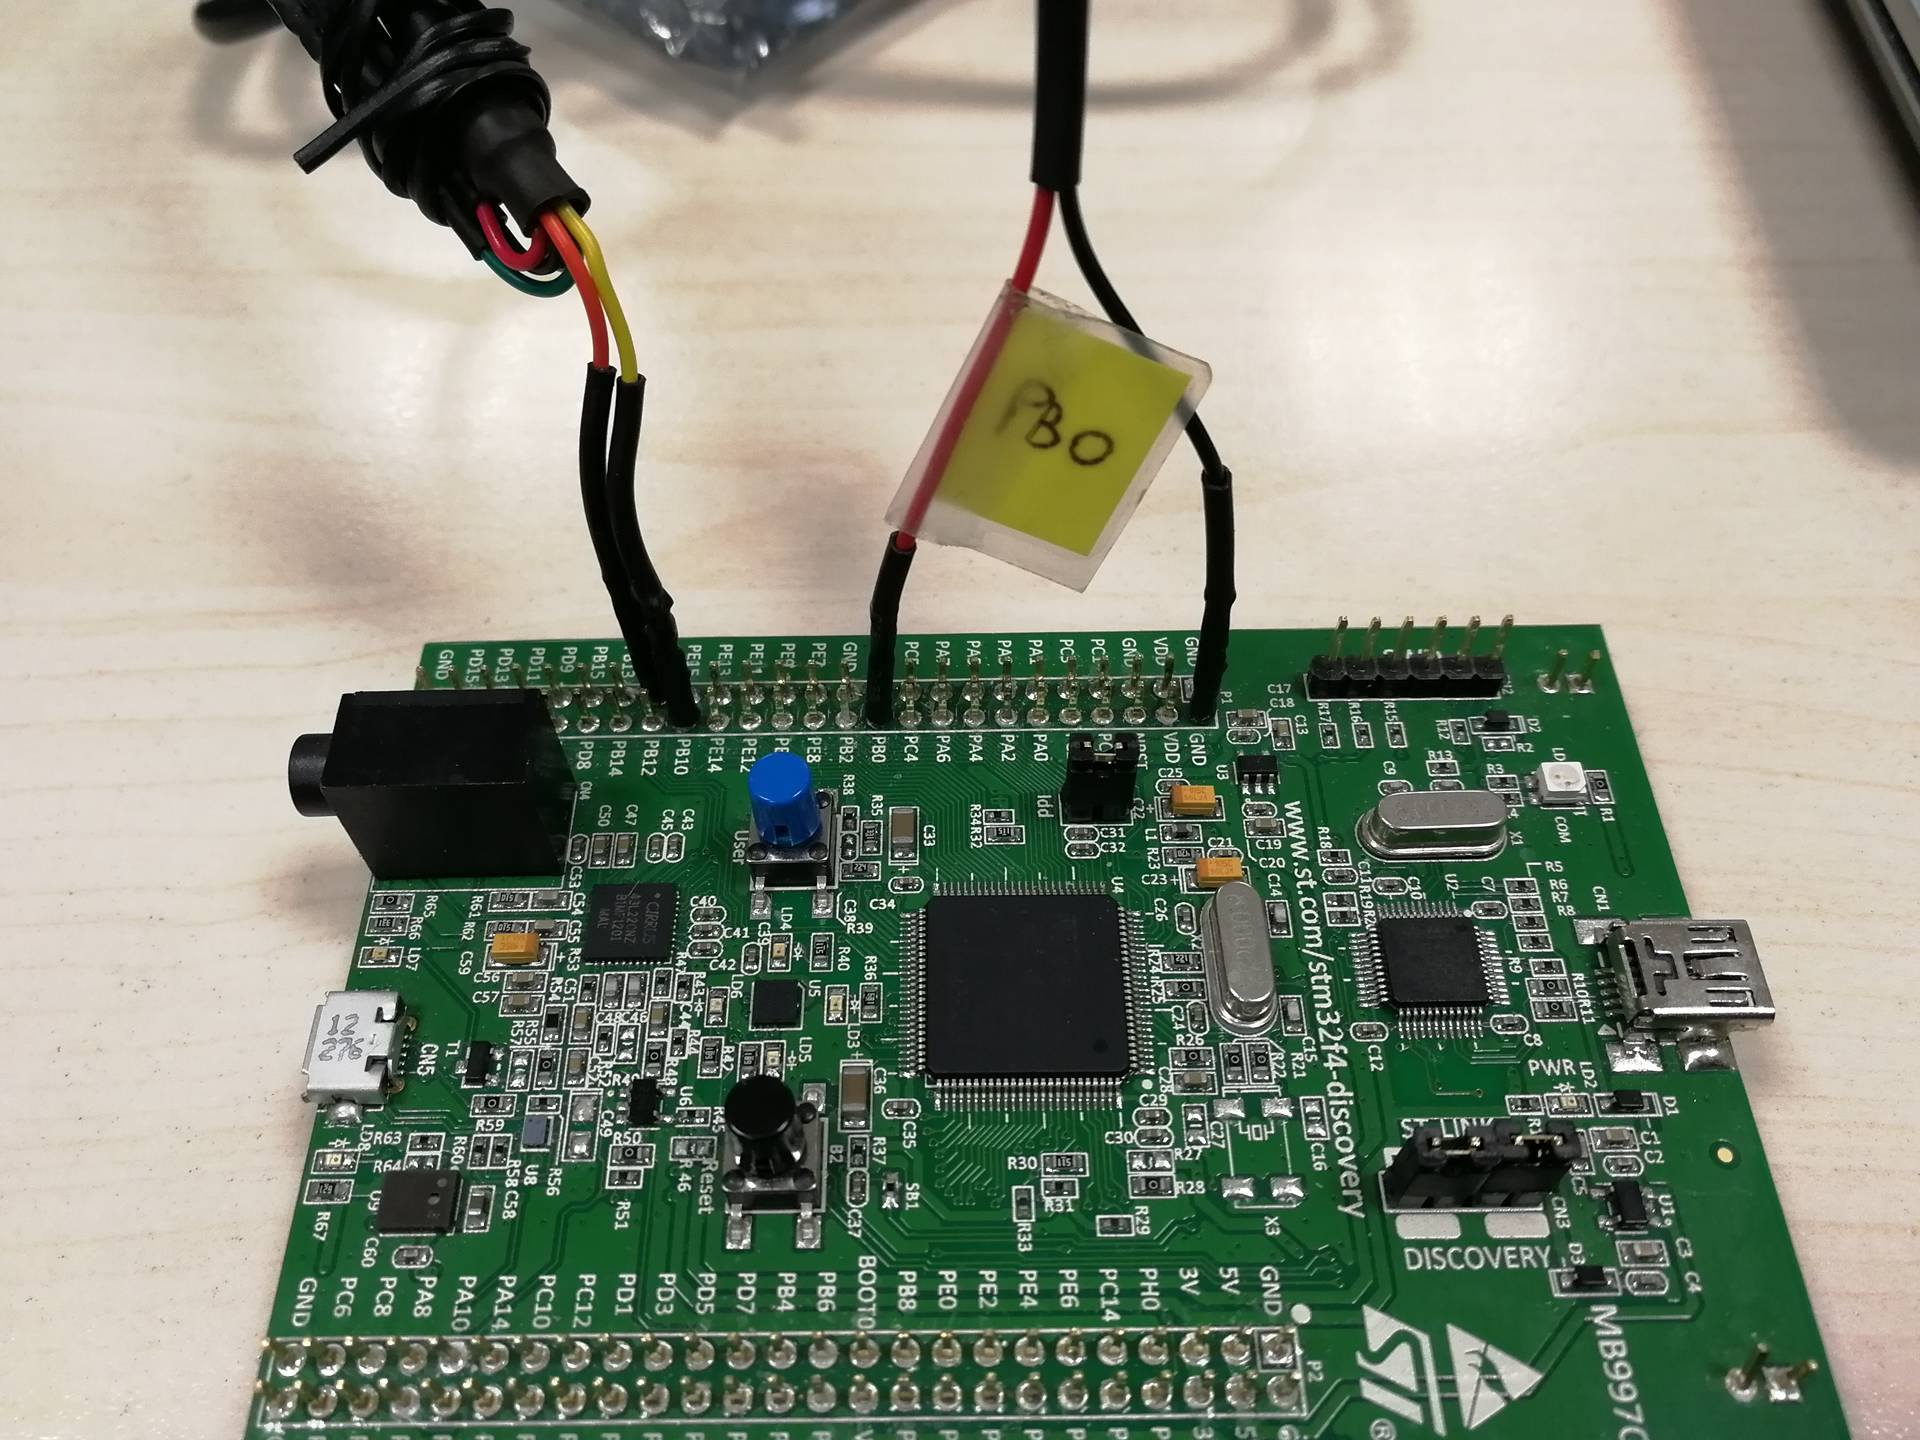
\includegraphics[width=1\textwidth]{./figures/connections.jpg}
  \caption{Connections}
  \label{fig:connections}
\end{figure}

\section{Experimental evaluation}\label{Results}
%TODO Arno
\subsection{Experimental setup}
\subsection{Results}

\section{Conclusions}
%TODO Arno
